
\section{The Algorithm}
\label{sec:expts}

\subsection{Ants}
The algorithm works by employing ant-based mobile agents to traverse the network and attempt to find the least weight path across the network. It does so by mimicking the pheromone trails of ants. In the algorithm, an ant is deployed from each node once per time step. The ant chooses its destination in the network randomly, and then follows a path to that node by following the probabilities stored in each node. The tables include a row for each possible destination node and a column for each neighbor node. As an ant travels, it looks up the row of its destination node and chooses its next node based on the probabilities for each neighbor. When it visits a node, it also updates the probability table by changing the node the ant has just come from according to: $$p = \frac{p_{old} + \Delta p}{1 + \Delta p}$$ and decreases the rest of the probabilities according to: $$p = \frac{p_{old}}{1 + \Delta p}$$ where $\Delta p$ is a function of the age of the ant: $$\Delta p = \frac{0.08}{age} + 0.05$$ In order to simulate traffic on the network, ants are delayed in getting to nodes based on a function of the spare capaticy $s$ of the node: $$delay = 80e^{-0.075s}$$ When an ant is traveling between nodes, the age of the ant is determined by the delay function. This means that more congested nodes take longer for ants to get to, reducing their effect on the probability table.

\subsection{Call Routing}
Calls are routed between nodes based on the probability tables as well. Much like the ants, calls look at the row in the probability table that corresponds to the destination node. The call then chooses the largest probabillity in the neighbor nodes and chooses that neighbor as its next node. If at any point a call attempts to be routed through a node that has no spare capacity, the call is dropped.

\subsection{Parameters}
There are several parameters which we used in our experiment worth noting:\\

-The average length of a call is 170 time steps. We used a Gaussian distribution with a mean of 170 and a standard deviation of 20 to model this.\\

-On average, one call is made every time step.\\

-One ant is released from each node at every time step.\\

-The maximum load on each node is 40 calls.\\

-Calls are made based on a uniform distribution of source and destination nodes.\\

-The graph used to model the network is the British Telecommunications core network circa 1996.\\

\begin{figure}[htb]

  \centering
  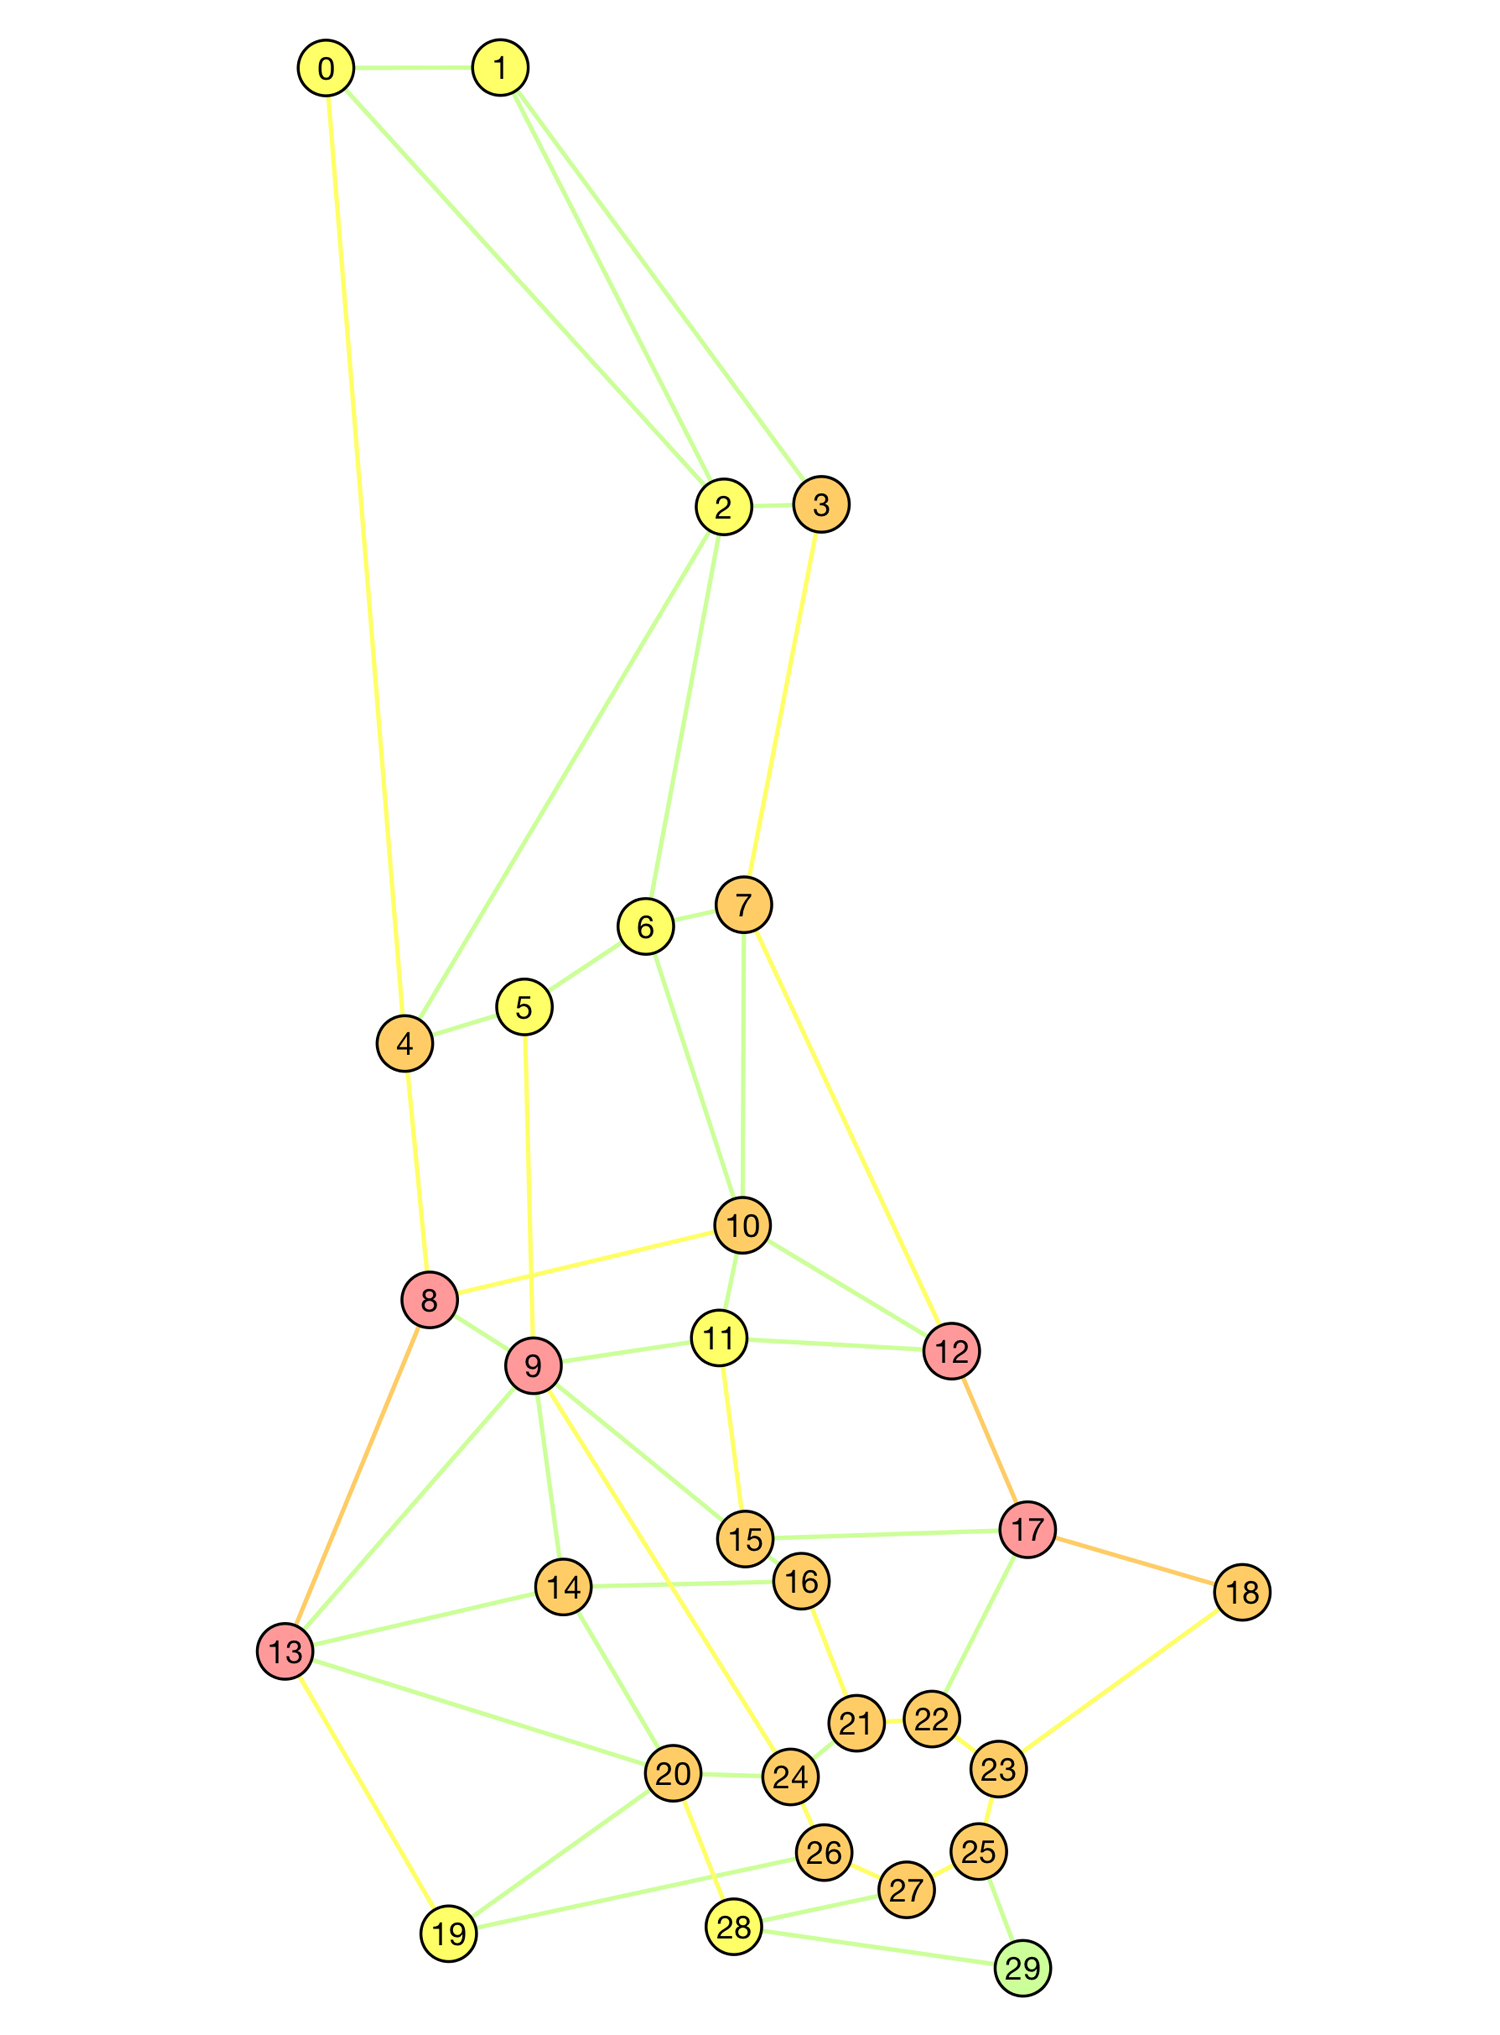
\includegraphics[width=0.47\textwidth]{figs/btc.jpg}
  \caption{A representation of the network being run by the ant-based algorithm at time $t = 10,000$.}
  \label{fig:btc}

\end{figure}

-The length of a run is 500 time steps for initialization (where no load is on the network) followed by 15,000 time steps with load for simulation.